[HOW DID THE TESTING GO??]

As mentioned in previous chapters, the primary metric for whether or not this implementation can be deemed effective is based upon the degree to which the severity of a participant's localisation errors decrease over time, if they decrease at all. This chapter will begin by investigating whether or not this is the case by reviewing the data captured during the listening tests. After this, further sections will investigate other conclusions or noteworthy observations that may be drawn from the additional data captured. Of particular interest is the aforementioned relationship between PCW adjustment and localisation, to this end I will be comparing PCW values and perceived/actual source positions before and after adjustment on an individual participant level.

\section{Localisation Error Over Time}
In order to properly analyse this metric I am looking at the average total error value for each of the eight source positions. This error value is the angular error that comes from subtracting the perceived source position from the actual source position. These two values are then made positive if either one is negative, so as to not produce deceptively low error values, and summed to produce a combined error value. This process is performed for every participant, and the mean error value for each measurement over the course of the test from each direction is then calculated based on that data. These mean error rates over time can then be plotted as in figure 4.1. 

\begin{figure}
	\caption{The average error rate over each direction.}
	\centering{
		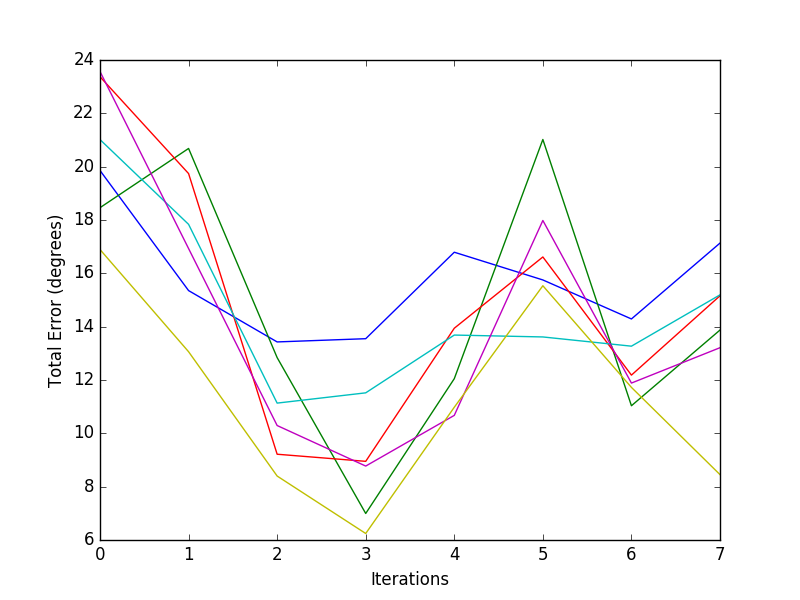
\includegraphics[scale=0.6]{average_error_each_direction}
	}
\end{figure}

On this chart each line represents a source position, so by following each line along it is simple to track how localisation errors for samples played from that source position changed over the course of the listening test. When displayed like this we can see something of a reduction in the overall errors for most source positions, but the short test length makes it unclear if these values would eventually begin to near zero. What we can see at play is the self-correcting quality afforded to the algorithm through knowledge of the history of previous changes. For almost all of the directions there are large spikes where the algorithm explores a sub-optimal child state and the participant's subsequent localisation attempt fares more poorly, in all cases but one (the black line representing the [-45.0, 135.0] source position) this mistake is quickly rectified as the algorithm makes adjustments in the opposite direction. If successive child states could be selected more intelligently, then it's quite possible that these kinds of mis-steps could be minimized further, reaching a more effectively individualised HRTF sooner.

It's worth noting that three of the four directions with the most promising results were situated in front of the participant: [-45.0, 45.0], [45.0, 45.0], and [-45.0, -45.0]. Suggesting a degree of front/back confusion in participants and a tendency towards assuming sources were positioned towards the front hemisphere of the test environment, leading to poor average error rates for sources positioned behind the participant. There is an exception to this in position [45.0, 135.0], which may have something to do with the starting HRTF used. Further research would be necessary to identify whether this is the case, but it would be interesting to try to assemble an ideal base HRTF to begin this process with. 

\section{Relationships Between PCs and Localisation Errors}
Again, starting with a description of how the data was was collated from the tests, and how it was arranged on the charts. I just can't yet work out the best way of displaying the data for this. It would be nice to represent it on a sphere or section of a sphere, something like that? 

\bigskip

same structure, charts in between 

\bigskip 

Conclusions we can draw, etc

\section{•}
Then this structure could be repeated as needed, for as much analysis as I get to do??